\chapter{Negative friction coefficient}\label{chap:negative_coef}

For the final part of this thesis, we concern ourselves with a proof of concept for a negative friction coefficient. From certain kirigami configurations, we have seen that stretching of the sheet can result in dramatic changes of the friction both with a positive and negative impact. By proposing a nanomachine coupling between normal load and such stretching we investigate the prospects of achieving a negative friction coefficient. 


\section{Nanomachine coupling}
We do not attempt to simulate the dynamics of any nanomachine, but we propose that a couplingg could be achieved, for instance by following a design as sketched in \cref{fig:nanomachine}. This could perhaps be achieved by rigging carbon nanotubes in a similar configuration. 

\begin{figure}[H]
  \centering
  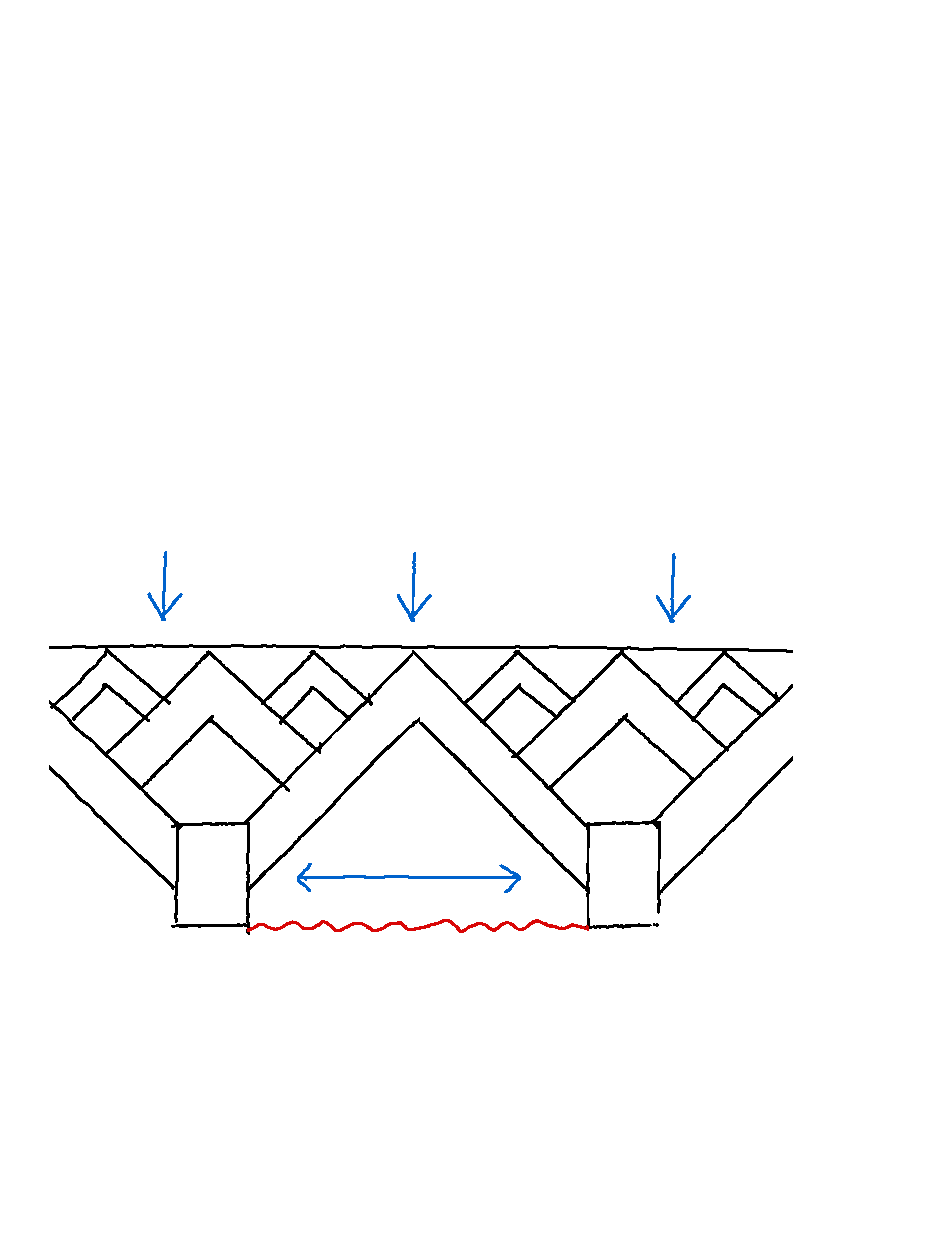
\includegraphics[width=0.5\linewidth]{figures/negative_coefficient/nanomachine.pdf}
  \caption{Working sketch for nanomachine}
  \label{fig:nanomachine}
\end{figure}

We mimic the coupling by implementing a tension force to our \acrshort{MD}
simulations. So far, we have kept the pull block at a fixed spacing throughout
the simulation, but now we keep the pull blocks apart by a tension force. The
tension force $F_t$ is modeled to be proportional to the normal load $F_t =
RF_N$ by a factor $R$ which represent the ratio of the load to stretching
coupling. We find that a ratio of $R=6$ will provide the necessary tension to
stretch the sheet to a rupture within the loading range that have used so far.
We use the Tetrahedron $(7,5,1)$ and Honeycomb $(2,2,1,5)$ from the pilot study
as an initial test as shown in \cref{fig:coupling_pop_7_5_1} and
\cref{fig:coupling_hon2215}. The results generally shows a good match to the
stretch curves generated in the pilot study which point to the fact that the
simultaneous loading and stretching did not suppress the non-linear effect. For
the Tetrahedon pattern this yields a quite good fit. For the Honeycomb pattern
however, we see that the tension vs.\ stretch curve breaks rapidly at around
\SI{0.75}{nN} of load (\SI{4.5}{nN} tension) transitioning from a stretch of
roughly 0.08 to 0.7. This made it difficult to actuallt capture any data point
in this stretch domain, and the ones added here yielded a higher friction than
otherwise suggested by the fixed stretch results from the pilot study. By
looking at the simulation frames (see \cref{sec:sheet_stretch}) we see
that this aligns well with the unfolding of the honeycomb pattern as all
Honeycomb units are flipped as the tension curve stabilizes again. This can be
explained by the fact the flipping each segment will require a minimum tension,
but as one segment is flipped one by one this unfolding will take place at more
or less a constant tension. 

This might be contributed to the 


\begin{figure}[H]
  \centering
  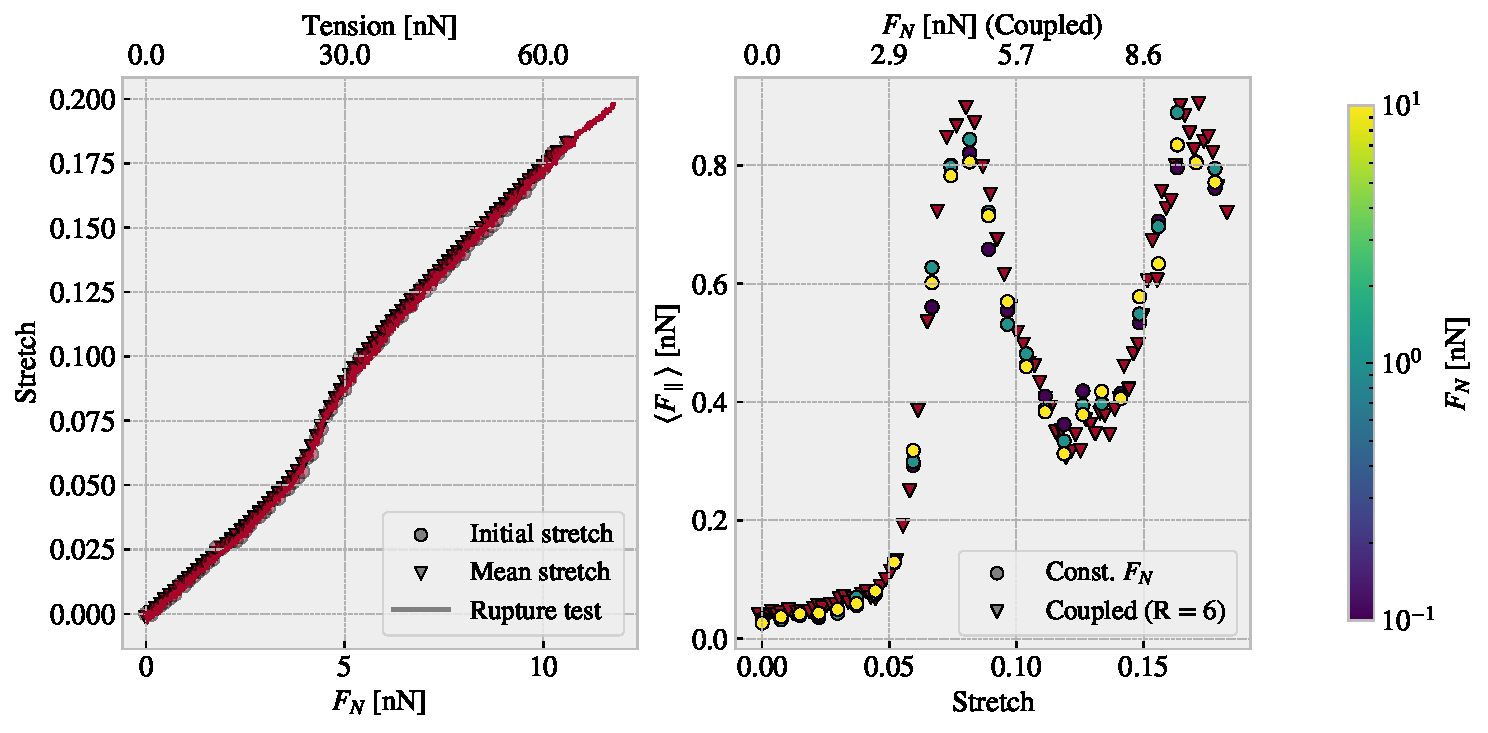
\includegraphics[width=0.9\linewidth]{figures/negative_coefficient/manual_coupling_free_pop7_5_1.pdf}
  \caption{\hl{Caption}}
  \label{fig:coupling_pop_7_5_1}
\end{figure}

\begin{figure}[H]
  \centering
  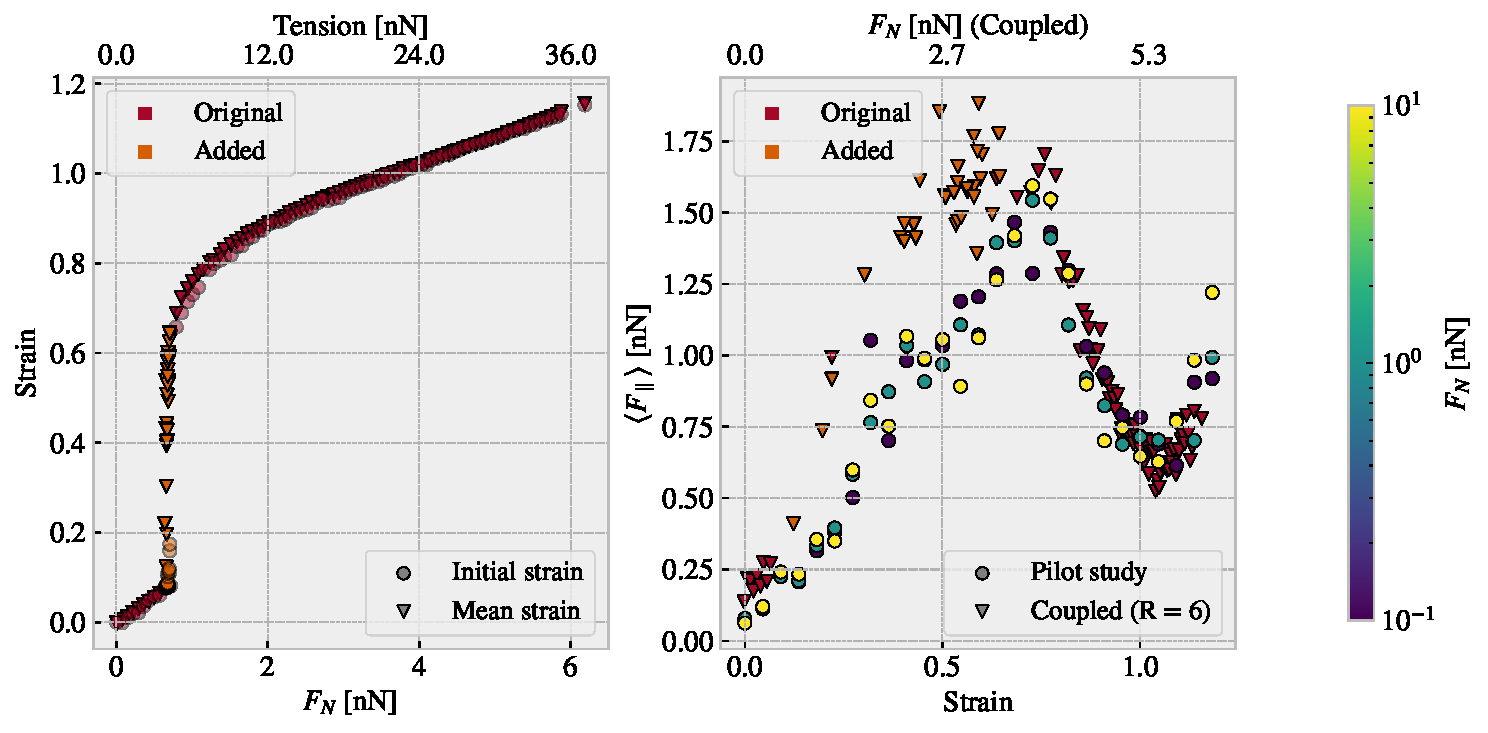
\includegraphics[width=0.9\linewidth]{figures/negative_coefficient/manual_coupling_free_hon2215.pdf}
  \caption{Caption}
  \label{fig:coupling_hon2215}
\end{figure}




% For the honeycomb we had to lower the stretch speed (from 0.001 to 0.0001, explain what it means) due to the very abrupt change in the stretch tension curve. 


